\documentclass[11pt]{article}

% Packages
\usepackage[utf8]{inputenc}
\usepackage[T1]{fontenc}
\usepackage[margin=0.8in]{geometry}
\usepackage{graphicx}
\usepackage{xcolor}
\usepackage{tikz}
\usepackage{enumitem}
\usepackage{amsmath}
\usepackage{amsfonts}
\usepackage{hyperref}

% Custom colors
\definecolor{primaryblue}{RGB}{41, 128, 185}
\definecolor{accentgreen}{RGB}{39, 174, 96}
\definecolor{warningorange}{RGB}{230, 126, 34}
\definecolor{darkgray}{RGB}{52, 73, 94}

% Custom formatting
\setlength{\parindent}{0pt}
\setlength{\parskip}{3pt}
\setlength{\baselineskip}{11pt}

% Header formatting
\usepackage{fancyhdr}
\pagestyle{fancy}
\fancyhf{}
\fancyhead[L]{\color{primaryblue}\textbf{DataMender Project Proposal}}
\fancyhead[R]{\color{darkgray}Group 8}
\fancyfoot[C]{\thepage}

\begin{document}

% Title section
\begin{center}
    {\LARGE\color{primaryblue}\textbf{DataMender: Smart Cleaning for Large CSV/Parquet Files}}
    
    \vspace{0.2cm}
    {\large\color{darkgray}Project Proposal}
    
    \vspace{0.3cm}
    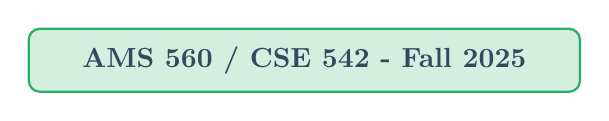
\begin{tikzpicture}
        \draw[accentgreen, thick, rounded corners, fill=accentgreen!20] (-3.5,-0.4) rectangle (3.5,0.4);
        \node[darkgray, font=\normalsize\bfseries] at (0,0) {AMS 560 / CSE 542 - Fall 2025};
    \end{tikzpicture}
    
    \vspace{0.3cm}
    {\color{darkgray}\textbf{Team:}} Ahmad Javadi Nezhad • Daniel Bazmandeh • Iliya Mirzaei • Nicholas Tardugno • Tamali Halder
    
    \vspace{0.2cm}
    {\color{darkgray}September 2025}
\end{center}

\vspace{0.3cm}

% Section 1: Problem and Motivation
\section{\color{primaryblue}Problem Statement and Motivation}

Data scientists spend 60-80\% of their time cleaning large datasets [5], yet existing tools cannot efficiently handle multi-gigabyte CSV/Parquet files with intelligent rule suggestions. Modern datasets suffer from inconsistent formatting (e.g., date formats like "2024-01-15", "01/15/2024", "15-Jan-2024"), complex missing value patterns, and sophisticated duplicate records requiring domain expertise to resolve correctly.

Current solutions force manual rule creation that doesn't scale to enterprise data volumes, creating critical bottlenecks in modern workflows. For example, cleaning a 10GB customer dataset with millions of records using traditional tools like OpenRefine [6] can take weeks of manual effort. This inefficiency leads to unreliable analytics, compromised ML models, and ultimately flawed business decisions. Organizations need automated, context-aware cleaning tools that maintain human oversight while processing enterprise-scale data efficiently.

% Section 2: Related Work and Gaps
\section{\color{primaryblue}Related Work and Current Limitations}

Recent research shows growing LLM application in data cleaning. Cocoon [3] performs semantic table profiling, AutoDCWorkflow [4] generates workflows automatically, LLMClean [1] creates context-aware rules, and DataCleanGPT [2] attempts general data standardization. However, these tools expose critical limitations: cannot handle multi-gigabyte files due to memory constraints and naive sampling strategies, provide limited human oversight mechanisms forcing risky automation choices, and lack robust safeguards against LLM hallucination where generated rules may introduce errors or violate data integrity requirements.

% Section 3: Solution Architecture
\section{\color{primaryblue}DataMender: Multi-LLM Data Cleaning System}

Our \textbf{novel contribution} is the first LLM ensemble system specifically designed for enterprise-scale data cleaning with comprehensive human validation workflows. DataMender introduces three key innovations for large-scale data processing.

\textbf{Scalable Data Profiler:} Uses optimized Pandas/Dask with stratified sampling that preserves statistical validity while handling datasets exceeding memory limits. Goes beyond basic statistics to identify cross-column relationships, data type inconsistencies, and pattern anomalies that inform targeted rule generation across diverse data domains.

\textbf{Multi-Model Rule Discovery Engine:} First system to employ GPT-5, GPT-4, Claude-3, and specialized local models in ensemble for data cleaning. Each model contributes unique strengths while cross-validation prevents hallucinations and provides quantitative confidence scores for generated cleaning rules.

\textbf{Interactive Validation Interface:} Validation workflow that integrates human expertise directly into the automation pipeline, ensuring generated transformations maintain data integrity and domain appropriateness across different use cases and industries.

% Section 4: Technical Innovation
\section{\color{primaryblue}Technical Innovation and Risk Mitigation}

\textbf{Sampling Strategy:} We develop a stratified sampling approach for LLM-based data cleaning that preserves statistical validity while ensuring representation of rare but important data patterns (outliers, edge cases, domain-specific anomalies). This enables LLM analysis of large datasets while maintaining data integrity across diverse domains, building upon recent advances in LLM-based data profiling [3].

\textbf{Comprehensive Hallucination Prevention:} Our five-layer framework prevents data-destructive errors: (1) Pattern-based confidence scoring across multiple data dimensions, (2) Multi-model validation including GPT-5 baseline comparisons, (3) Domain expert review workflow, (4) Complete operation logging for auditability, (5) Controlled testing on representative data samples matching real distributions. This addresses critical limitations identified in recent LLM cleaning research [1,2].

\textbf{Domain-Adaptive Rule Generation:} System dynamically adapts LLM prompts based on detected data characteristics (numerical, categorical, temporal, textual), ensuring generated cleaning rules are contextually appropriate regardless of the specific domain or industry application, extending techniques from AutoDCWorkflow [4].

% Section 5: Competitive Analysis
\section{\color{primaryblue}Competitive Position}

\begin{table}[h]
\centering
\footnotesize
\begin{tabular}{|l|p{2.2cm}|p{2.2cm}|p{2.8cm}|}
\hline
\textbf{Feature} & \textbf{OpenRefine} & \textbf{Trifacta/Alteryx} & \textbf{DataMender} \\
\hline
\textbf{Rule Generation} & Manual only & Template-based & \textbf{Full LLM automation} \\
\hline
\textbf{Scale Support} & Memory-limited & Enterprise only & \textbf{Multi-GB optimized} \\
\hline
\textbf{Validation} & Basic preview & Enterprise workflow & \textbf{AI-assisted validation} \\
\hline
\textbf{Error Prevention} & User experience & Basic testing & \textbf{Multi-model mitigation} \\
\hline
\textbf{Cost} & Free & Expensive & \textbf{Open-source} \\
\hline
\end{tabular}
\caption{Competitive feature comparison}
\label{tab:comparison}
\end{table}

% Section 6: Implementation and Deliverables
\section{\color{primaryblue}Implementation Plan}

\textbf{8-Week Schedule:} Foundation (weeks 1-2): dataset curation and profiler. Intelligence (weeks 3-4): multi-LLM ensemble with GPT-5 baseline. Scale (weeks 5-6): multi-gigabyte processing optimization. Validation (weeks 7-8): testing and documentation.

\textbf{Deliverables:} Working data cleaning tool, YAML configuration system, demonstration video with million-record processing, technical report with performance metrics and validation results.

\textbf{Team Roles:} Ahmad: multi-LLM integration. Daniel: scalable profiling. Iliya: validation workflows. Nicholas: batch processing engine. Tamali: testing and validation.

% References
\section{\color{primaryblue}References}

\begin{enumerate}[itemsep=1pt]
\item Biester, L., et al. (2024). LLMClean: Context-Aware Tabular Data Cleaning via LLM-Generated OFDs. \textit{arXiv:2404.18681}.
\item Chen, J., et al. (2023). RetClean: Retrieval-Based Data Cleaning Using LLMs and Data Lakes. \textit{arXiv:2303.16909}.
\item Huang, J., \& Wu, Y. (2024). Cocoon: Semantic Table Profiling Using Large Language Models. \textit{arXiv:2410.15547}.
\item Li, X., et al. (2024). AutoDCWorkflow: LLM-based Data Cleaning Workflow Auto-Generation. \textit{arXiv:2412.06724}.
\item OpenRefine. (2024). Documentation. https://openrefine.org/docs/
\item Trifacta. (2024). Predictive Transformation Overview. https://docs.trifacta.com/
\end{enumerate}

\end{document}